%=================================================================
% IEEE "RECIPE-STYLE" TEMPLATE -- LabDST
%=================================================================
% What this is:
%   This template uses the CLASS and SYNTAX of IEEEtran (the same
%   one IEEE itself uses), but organizes the content with the KEY
%   SECTION STRUCTURE that MDPI uses (Introduction, Materials and
%   Methods, Design and Implementation, Results, Discussion,
%   Conclusions), because that structure explicitly explains WHAT
%   each section must contain -- not just how the LaTeX code works.
%
% Language:
%   The paper must be written entirely in English. This was decided
%   so the work can reach an international audience and match the
%   language IEEE venues expect. Keep the whole document in a single
%   language -- do not mix English and Spanish anywhere in the file,
%   including these instructions, figure/table captions, and code
%   comments.
%
% How to use it:
%   1. Every section below already contains guidance text explaining
%      what should go in that part of the paper. Replace it with your
%      actual content as you write.
%   2. The example figure uses fig1.png (already included in this
%      same folder). Replace it with your own figure, or add more
%      figures using the same block as a model.
%   3. The bibliography is EXTERNAL: it is defined in bibliography.bib
%      (in this same folder), and sources are cited with \cite{key}.
%      Do not type references by hand inside the .tex file.
%   4. Compile with pdflatex + bibtex/biber + pdflatex + pdflatex
%      (or "latexmk -pdf") so citations and the bibliography are
%      generated correctly.
%   5. Delete Section 0 ("How to Use This Template") completely
%      before submitting the final version: it is instructional only
%      and must not appear in the finished paper.
%=================================================================

\documentclass[lettersize,journal]{IEEEtran}
%--------------------
% Most common class options (uncomment/change as needed):
%--------------------
% [journal]     -> journal article (default format of this template)
% [conference]  -> conference paper
% [10pt,journal,compsoc] -> Computer Society journal article
% [9pt,technote]         -> brief note / correspondence
% Full option reference: see "IEEE Paper Template/main.tex"
% (the official IEEEtran guide) in the sibling folder of this template.

\usepackage{amsmath,amsfonts}
\usepackage{array}
\usepackage[caption=false,font=normalsize,labelfont=sf,textfont=sf]{subfig}
\usepackage{textcomp}
\usepackage{stfloats}
\usepackage{url}
\usepackage{graphicx}
\usepackage{cite}
\usepackage{xcolor}
\hyphenation{op-tical net-works semi-conduc-tor IEEE-Xplore}
\def\BibTeX{{\rm B\kern-.05em{\sc i\kern-.025em b}\kern-.08em
    T\kern-.1667em\lower.7ex\hbox{E}\kern-.125emX}}
\usepackage{balance}

\begin{document}

%=================================================================
% Title: it should be clear, specific, and avoid mathematical or
% chemical formulas whenever possible. A good title lets someone
% outside the project understand what the work is about without
% reading the rest of the document.
\title{Title}

\author{Student 1, Student 2, Student 3, Student 4, Student 5, Jorge A. Lizarraga, Graciela Baca, Luis Enrique González-Jiménez and Luis F. Luque-Vega
\thanks{The authors are with the Department of Technological and
Industrial Processes, ITESO, Tlaquepaque 45604, Jalisco, Mexico.}}

\markboth{Name of the project or of the journal/course}%
{Lizarraga \MakeLowercase{\textit{et al.}}: Short paper title}

\maketitle

%=================================================================
\begin{abstract}
The abstract is a single paragraph of 150--250 words, written last,
once results already exist. It must be an objective synthesis of the
whole paper, without stating conclusions that are not supported in the
body of the text. Even though it has no visible subheadings, draft it
following this internal structure: \\
(1) \textbf{Context}: what question or need motivates the work? \\
(2) \textbf{Methods}: what was done to address it? (approach,
materials, main methods, in 1-2 lines). \\
(3) \textbf{Results}: what was found? (the main findings, with
concrete data if possible). \\
(4) \textbf{Conclusion}: what does that finding imply? \\
Avoid mathematical or chemical formulas inside the abstract.
\end{abstract}

\begin{IEEEkeywords}
keyword 1, keyword 2, keyword 3 (3 to 6 terms specific to the
topic of the paper, yet reasonably common within the discipline --
they help other researchers find the work).
\end{IEEEkeywords}

%=================================================================
\setcounter{section}{-1} %% Delete this section together with this line before submitting.
\section{How to Use This Template}

This section is instructional only: delete it completely (together
with \texttt{\textbackslash setcounter\{section\}\{-1\}}) before the
final submission, and start numbering from Section 1 (Introduction).

The order and names of the following sections are the ones IEEE uses
most often for technical and research papers, adapted so that each
heading explicitly states what content belongs inside it -- so there
is no need to guess what to write in each part. If your journal,
conference, or course requires a different order, follow those
specific instructions; the structure here is a starting point, not a
rigid rule.

%=================================================================
\section{Introduction}

% IEEE journal papers open the first paragraph with a drop-cap letter
% via \IEEEPARstart. Keep this wrapper when you replace the guidance
% text below with your actual first paragraph.
\IEEEPARstart{T}{he} introduction should place the work in a broad
context and explain why it matters. It should cover, in this order:
\begin{itemize}
\item The problem or question that motivates the work, explained so
that someone outside the specific field can understand it.
\item The \textbf{motivation}: why this problem matters, who is
affected by it, and what happens if it is not addressed.
\item A brief preview that related work is reviewed next (the actual
review goes in the Related Work subsection below).
\item The gap, limitation, or open controversy that the reviewed
related work leaves unresolved, and that this paper addresses.
\item The concrete objective of the work.
\item A preview of the main conclusion (one or two sentences).
\end{itemize}
Citation example: citing a source \cite{placeholder2026}. To cite
several sources at once: \cite{placeholder2026,placeholder-conf-2026}.
A closing paragraph that "summarizes the structure of the paper" is
not required unless your journal/course explicitly asks for it.

\subsection{Related Work}

Summarize the state of the art relevant to this paper: similar
robots or devices, similar methodologies, or comparable solutions
already reported in the literature. For each relevant reference,
briefly state what it solved and what it left open, citing the source
with \textbackslash cite\{\}. Close the subsection by clarifying how
this work differs from, extends, or builds on that prior work -- this
is what justifies the contribution claimed in the objective above.

%=================================================================
\section{Materials and Methods}
\label{sec:methods}

This section must have enough detail for someone else to replicate
the work. Include, as applicable:
\begin{itemize}
\item The materials, components, equipment, datasets, or tools used,
with relevant specifications (well-established methods do not need to
be justified in detail; citing them is enough).
\item The methods or procedures applied, described with enough detail
to be reproducible. If a method is new, describe it in detail; if it
is a known method, a citation plus a brief description is enough.
\item If the work uses public data or generates its own dataset,
state where it is available (or state that it will be provided during
review).
\item If the work involves human or animal subjects, or requires
ethical approval, state the authority that granted it and the
approval code. If not applicable, this can be omitted.
\item If generative artificial intelligence was used (beyond
superficial text editing) to generate text, data, or graphics, or to
support the study design, data collection, or analysis, disclose it
briefly here.
\end{itemize}

\begin{quote}
Example of a long quotation or of a highlighted note within the
text (use this \texttt{quote} block sparingly).
\end{quote}

%=================================================================
\section{Design and Implementation of the Technological Solution}
\label{sec:design}

This section shows how the methods and materials from the
previous section were turned into the actual built solution. Include,
as applicable:
\begin{itemize}
\item The overall system architecture (block diagram) showing how
the different subsystems interact.
\item Mechanical, electronic, and/or software design decisions, with
enough detail to be reproducible.
\item How the different subsystems were integrated into the complete
solution.
\item Configuration, calibration, or programming steps needed to
bring the system into working operation.
\end{itemize}
Use figures (block diagrams, CAD renders, architecture diagrams,
photographs of the assembled system) and tables to support this
description, following the same figure/table conventions shown in the
Results section below.

%=================================================================
\section{Results}

This section presents the findings concisely and precisely,
without interpreting them in depth yet (that interpretation belongs in
Discussion). It may be divided into subsections if the work covers
several experiments or stages of results.

\subsection{Example subsection}
\subsubsection{Example subsubsection}

Bulleted lists look like this:
\begin{itemize}
\item First point;
\item Second point;
\item Third point.
\end{itemize}

Numbered lists look like this:
\begin{enumerate}
\item First item;
\item Second item;
\item Third item.
\end{enumerate}

\subsection{Figures and Tables}

All figures and tables must be cited in the text before they
appear, for example: Figure~\ref{fig1} shows... or Table~\ref{tab1}
summarizes...

\begin{figure}[!t]
\centering
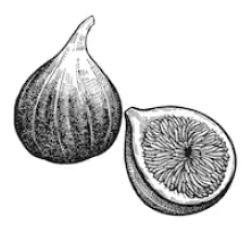
\includegraphics[width=2.5in]{fig1}
\caption{Brief description of what the figure shows. The caption
must be understandable without reading the main text.}
\label{fig1}
\end{figure}

\begin{table}[!t]
\centering
\caption{Brief description of what the table shows.}
\label{tab1}
\begin{tabular}{|c|c|c|}
\hline
\textbf{Title 1} & \textbf{Title 2} & \textbf{Title 3} \\
\hline
Data & Data & Data \\
\hline
Data & Data & Data \\
\hline
\end{tabular}
\end{table}

Example of a figure with several panels (a, b, c...), useful when
several related images must be presented together:
\begin{figure}[!t]
\centering
\subfloat[Description of panel (a).]{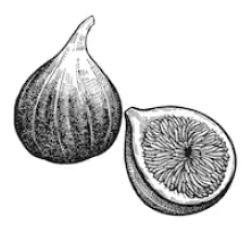
\includegraphics[width=1.1in]{fig1}}
\hfil
\subfloat[Description of panel (b).]{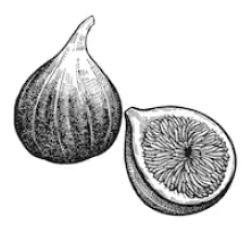
\includegraphics[width=1.1in]{fig1}}
\caption{General description covering both panels. (a) Explanation
of panel (a). (b) Explanation of panel (b).}
\label{fig2}
\end{figure}

\subsection{Equations}

Equations are numbered consecutively throughout the whole paper:
(1), (2), (3)... Do not use roman numerals or section numbers to
number them. Example:
\begin{equation}
\label{eq:example}
y = \sum_{i=0}^{n} a_i x^i.
\end{equation}
To reference it in the text: see Eq.~(\ref{eq:example}).

%=================================================================
\section{Discussion}

This is where the results are interpreted, not just repeated. It
should answer:
\begin{itemize}
\item What do the obtained results mean?
\item How do they compare with the state of the art cited in the
introduction? Do they confirm, contradict, or qualify previous work?
\item What limitations does the work have (methodological, of scope,
of validity)?
\item What practical or theoretical implications does the finding
have?
\item What future work does this open up?
\end{itemize}
This section can be merged with Results if your journal/course prefers
that (check the specific instructions), but keeping them separate is
recommended to avoid mixing "what was found" with "what it means".

%=================================================================
\section{Conclusions}

A brief synthesis (not a repetition of the abstract or of the
discussion) of the answer to the question posed in the introduction,
and of the concrete contribution of the work. This section is not
mandatory if the discussion already provides that closure, but it is
recommended when the paper is long or the discussion covered several
topics.

%=================================================================
%% Back matter sections. IEEE does not require special macros for
%% this -- they are simple unnumbered sections before Acknowledgment.
%% Include them when your journal/course requires them; if they do
%% not apply, they can be omitted or left as "Not applicable".

\section*{Author Contributions}
If the paper has several authors, briefly specify each person's
individual contribution (e.g., conceptualization, methodology,
software, validation, formal analysis, investigation, resources, data
curation, writing, visualization, supervision, project administration,
funding acquisition). Authorship must be limited to those who
contributed substantially to the reported work.

\section*{Data Availability}
State where the data, code, or materials that support the reported
results can be found (repository, link, DOI). If no new data were
generated, or if there are privacy or confidentiality restrictions,
state that as well.

\section*{Acknowledgment}
Acknowledge people or institutions that supported the work but do
not qualify as authors (technical or administrative support, in-kind
donations, funding). If generative AI was used in preparing the
manuscript, disclose it here with the tool name, version, and the
specific use it was given.

\section*{Conflicts of Interest}
Choose whichever of the following applies, or adapt it to your
case: \\
\textbullet\ \textbf{No conflict}: state ``The authors declare no
conflicts of interest.'' \\
\textbullet\ \textbf{Declared conflict}: identify and declare any
personal circumstances or interests that could be perceived as
inappropriately influencing the representation or interpretation of
the reported results. \\
\textbullet\ \textbf{Role of funders}: state the role of any funders
in the design of the study; in the collection, analyses, or
interpretation of data; in the writing of the manuscript; or in the
decision to publish the results. If there was no such role, state:
``The funders had no role in the design of the study; in the
collection, analyses, or interpretation of data; in the writing of the
manuscript; or in the decision to publish the results.''

%=================================================================
\balance

\bibliographystyle{IEEEtran}
\bibliography{bibliography}

%=================================================================
%% Optional appendix -- uncomment if needed.
%\appendix
%\section{Appendix title}
%Supplementary content that is not central to the body of the
%paper, but is necessary to reproduce or dive deeper into it (e.g.,
%long mathematical derivations, raw data, code). Appendix figures and
%tables are numbered as Figure A1, Table A1, etc., and must be cited
%in the main text.

%=================================================================
%% Author biographies (optional, common in some IEEE journals).
%\begin{IEEEbiographynophoto}{First Last}
%Brief biography without a photo: education, research interests.
%\end{IEEEbiographynophoto}
%
%\begin{IEEEbiography}[{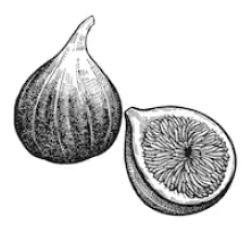
\includegraphics[width=1in,height=1.25in,clip,keepaspectratio]{fig1}}]{First Last}
%Brief biography with a photo: education, research interests.
%\end{IEEEbiography}

\end{document}
